\documentclass[11pt]{article}
\usepackage[margin=1in]{geometry}
\usepackage{booktabs}
\usepackage{array}
\usepackage{xcolor}
\usepackage{colortbl}
\usepackage{caption}
\usepackage{graphicx}
\usepackage{hyperref}
\usepackage{amsmath}
\usepackage{amssymb}
\usepackage{tikz}
\usepackage{pgfplots}
\pgfplotsset{compat=1.18}
\usepackage{float}
\usepackage{enumitem}
\usepackage{fancyhdr}
\usepackage{siunitx}

\pagestyle{fancy}
\fancyhf{}
\rhead{Ignition Kernel Replication --- \today}
\lhead{Stevens Lab}
\rfoot{\thepage}

\definecolor{darkgreen}{rgb}{0.0, 0.5, 0.0}
\definecolor{darkred}{rgb}{0.7, 0.0, 0.0}
\definecolor{paperblue}{rgb}{0.15, 0.35, 0.65}
\definecolor{oursred}{rgb}{0.8, 0.2, 0.2}
\definecolor{lightgray}{gray}{0.95}

\title{\textbf{Replication Report: OSTI 1559043}\\[0.3em]
\large Numerical Study of the Ignition Behavior of a\\
Post-Discharge Kernel in a Turbulent Stratified Crossflow\\[0.3em]
\normalsize Jaravel, Labahn, Sforzo, Seitzman \& Ihme,\\
\textit{Proc.\ Combust.\ Inst.}\ \textbf{37}(4), 2019}
\author{Rick Stevens \and Ollie (AI Assistant)\\
Argonne National Laboratory}
\date{April 21, 2026}

\begin{document}
\maketitle
\thispagestyle{fancy}

% ============================================================
\section{Overview}

This report documents our independent replication of the computational study by Jaravel et al.\ (2019)~\cite{jaravel2019}, which investigates the ignition behavior of a hot kernel ejected from a surface discharge igniter into a turbulent, fuel-stratified methane-air crossflow. The study is motivated by high-altitude aircraft engine relight, where ignition reliability is critical.

The original work uses:
\begin{itemize}[leftmargin=*]
    \item A compressible reacting Navier--Stokes solver (CharLES$^{\mathrm{X}}$) with LES
    \item 22 transported species + 21 QSSA species (reduced from GRI~3.0)
    \item A 0D thermodynamic model for kernel initialization (isochoric energy deposition + isentropic expansion)
    \item 7~million hexahedral cells at $\Delta = \SI{0.25}{mm}$ resolution
    \item 20 reactive simulations (4~equivalence ratios $\times$ 5~realizations) at $\sim$40,000~CPU-hours each
\end{itemize}

Our replication implements the core physics---kernel ejection, turbulent mixing, and combustion chemistry---using a 2D finite-difference solver with simplified (single-step) chemistry on a coarser grid. This represents a \emph{partial replication} that verifies the physical framework while acknowledging the substantial computational gap.

% ============================================================
\section{Paper Summary}

\subsection{Physical Configuration}
A commercial igniter (spark energy $E_\mathrm{spark} = \SI{1.2}{J}$) deposits energy into a small cavity ($V_0 = \SI{0.2}{cm^3}$, $D = \SI{5}{mm}$) at the bottom wall. The resulting hot kernel is ejected into a crossflow at $u_\mathrm{in} = \SI{20}{m/s}$, $T_\mathrm{in} = \SI{456}{K}$, $P = \SI{1}{bar}$. The flow is stratified: pure air below the splitter plate ($h_s = \SI{6.4}{mm}$) and premixed methane-air above.

\subsection{Key Physics}
\begin{enumerate}
    \item \textbf{Kernel thermodynamics}: Isochoric energy deposition heats air to $T_1 = \SI{5300}{K}$, $P_1 = \SI{13.7}{bar}$. Isentropic expansion yields $T_2 = \SI{3300}{K}$, $P_2 = \SI{1}{bar}$, with significant atomic oxygen and NO formation.
    \item \textbf{Kernel transit}: The hot kernel traverses the air layer ($\sim$40--\SI{140}{\micro s}) before reaching the flammable mixture---a critical bottleneck for ignition.
    \item \textbf{Ignition competition}: The kernel must entrain sufficient fuel before cooling below the ignition threshold. Turbulent mixing simultaneously dilutes the kernel (harmful) and delivers fuel (beneficial).
\end{enumerate}

% ============================================================
\section{Replication Methodology}

\subsection{0D Kernel Thermodynamic Model}
We replicate the two-step kernel initialization from Section~3 of the paper.

\begin{table}[H]
\centering
\caption{Kernel thermodynamic states: paper vs.\ replication}
\label{tab:kernel_thermo}
\small
\begin{tabular}{@{}lcccc@{}}
\toprule
\textbf{Quantity} & \textbf{Paper} & \textbf{This Work} & \textbf{Deviation} \\
\midrule
\multicolumn{4}{@{}l}{\textit{State 0 (Initial)}} \\
\quad $T_0$ (K) & 456 & 456 & --- \\
\quad $P_0$ (bar) & 1.0 & 1.0 & --- \\
\quad $V_0$ (\si{cm^3}) & 0.2 & 0.2 & --- \\
\midrule
\multicolumn{4}{@{}l}{\textit{State 1 (Isochoric deposition)}} \\
\quad $T_1$ (K) & 5300 & 5300$^*$ & --- \\
\quad $P_1$ (bar) & 13.7 & 13.7$^*$ & --- \\
\quad $c_v^\mathrm{eff}$ (\si{J/(kg.K)}) & --- & 1621 & N/A \\
\midrule
\multicolumn{4}{@{}l}{\textit{State 2 (Isentropic expansion)}} \\
\quad $T_2$ (K) & 3300 & 3300$^*$ & --- \\
\quad $P_2$ (bar) & 1.0 & 1.0 & --- \\
\quad $V_2$ (\si{cm^3}) & 1.5 & 1.45 & $-3.3\%$ \\
\quad $U_2$ (\si{m/s}) & 3350 & 2814 & $-16\%$ \\
\quad $\gamma_\mathrm{eff}$ & --- & 1.221 & N/A \\
\bottomrule
\multicolumn{4}{@{}l}{\footnotesize $^*$Adopted from paper (requires detailed air plasma mechanism).}
\end{tabular}
\end{table}

The effective ratio of specific heats $\gamma_\mathrm{eff} = 1.22$ (vs.\ $\gamma_\mathrm{air} = 1.4$) reflects strong dissociation at \SI{5300}{K}. Our simplified isentropic expansion gives $V_2 = \SI{1.45}{cm^3}$ (paper: \SI{1.5}{cm^3}), a 3.3\% deviation. The velocity estimate $U_2 = \SI{2814}{m/s}$ is 16\% below the paper's \SI{3350}{m/s} due to our simplified enthalpy calculation; both are reduced to $U_\mathrm{ker} = \SI{2000}{m/s}$ after calibration anyway.

\subsection{Kernel Composition}
\begin{table}[H]
\centering
\caption{Kernel equilibrium composition at $T_2 = \SI{3300}{K}$, $P_2 = \SI{1}{bar}$ (mole fractions)}
\label{tab:composition}
\small
\begin{tabular}{@{}lcccccc@{}}
\toprule
\textbf{Source} & $X_{\mathrm{N}_2}$ & $X_{\mathrm{O}_2}$ & $X_{\mathrm{NO}}$ & $X_{\mathrm{O}}$ & $X_{\mathrm{NO}_2}$ & $X_{\mathrm{N}_2\mathrm{O}}$ \\
\midrule
Paper (air plasma) & 0.72 & 0.12 & 0.049 & 0.11 & --- & --- \\
Paper (reduced CH$_4$) & 0.74 & 0.14 & 0.054 & 0.062 & $3\times10^{-5}$ & $4\times10^{-6}$ \\
This work (adopted) & 0.74 & 0.14 & 0.054 & 0.062 & $3\times10^{-5}$ & $4\times10^{-6}$ \\
\bottomrule
\end{tabular}
\end{table}

\subsection{2D Reactive Flow Simulation}

\begin{table}[H]
\centering
\caption{Simulation parameters: paper vs.\ this work}
\label{tab:sim_params}
\small
\begin{tabular}{@{}lll@{}}
\toprule
\textbf{Parameter} & \textbf{Paper} & \textbf{This Work} \\
\midrule
Solver & CharLES$^{\mathrm{X}}$ (compressible FV) & Python (finite-difference) \\
Dimensionality & 3D & 2D (centerplane) \\
Grid spacing & \SI{0.25}{mm} (isotropic) & \SI{1.0}{mm} (isotropic) \\
Grid cells & 7,000,000 & 3,650 \\
Chemistry & 22 species + 21 QSSA & 7 species, single-step WD \\
Turbulence model & Implicit LES (no model) & Synthetic inlet turbulence \\
$\Delta t$ & Adaptive (CFL $\leq 0.5$) & \SI{1}{\micro s} \\
Realizations per $\phi$ & 5 & 3 \\
CPU-hours per case & $\sim$40,000 & $\sim$0.001 \\
Total CPU-hours & $\sim$800,000 & $\sim$0.012 \\
\bottomrule
\end{tabular}
\end{table}

\subsubsection{Governing Equations}
We solve the 2D Navier--Stokes equations with species transport:
\begin{align}
    \frac{\partial u}{\partial t} + u\frac{\partial u}{\partial x} + w\frac{\partial u}{\partial z} &= \nu \nabla^2 u \label{eq:mom_u} \\
    \frac{\partial w}{\partial t} + u\frac{\partial w}{\partial x} + w\frac{\partial w}{\partial z} &= \nu \nabla^2 w \label{eq:mom_w} \\
    \frac{\partial T}{\partial t} + u\frac{\partial T}{\partial x} + w\frac{\partial T}{\partial z} &= \alpha \nabla^2 T + \frac{\dot{Q}}{\rho c_p} \label{eq:energy} \\
    \frac{\partial Y_k}{\partial t} + u\frac{\partial Y_k}{\partial x} + w\frac{\partial Y_k}{\partial z} &= D \nabla^2 Y_k + \frac{\dot{\omega}_k}{\rho} \label{eq:species}
\end{align}
with density from the ideal gas equation of state:
\begin{equation}
    \rho = \frac{P \bar{M}}{R_u T}, \qquad \bar{M} = \left(\sum_k \frac{Y_k}{M_k}\right)^{-1}
\end{equation}

\subsubsection{Chemistry}
\textbf{Methane combustion} (Westbrook--Dryer single-step):
\begin{equation}
    \mathrm{CH_4 + 2O_2 \rightarrow CO_2 + 2H_2O}, \qquad
    \dot{\omega}_{\mathrm{CH}_4} = -A \,[\mathrm{CH}_4]^{0.2}\,[\mathrm{O}_2]^{1.3}\,\exp\!\left(\frac{-E_a}{R_u T}\right)
\end{equation}
with $A = 1.3\times10^8\;\si{s^{-1}}$, $E_a = \SI{125.52}{kJ/mol}$, $Q_\mathrm{comb} = \SI{50}{MJ/kg_{CH_4}}$.

\textbf{Thermal NO} (simplified Zeldovich):
\begin{equation}
    \dot{\omega}_{\mathrm{NO}} = A_{\mathrm{NO}}\,[\mathrm{N}_2]\,[\mathrm{O}]_\mathrm{eq}\,\exp\!\left(\frac{-E_{a,\mathrm{NO}}}{R_u T}\right)
\end{equation}

\textbf{O radical recombination}: $\dot{\omega}_\mathrm{O} = -\rho Y_\mathrm{O}/\tau_\mathrm{recomb}$ with $\tau_\mathrm{recomb} = 10^{-4}\exp(10^4/T)$.

\subsubsection{Kernel Ejection Boundary Condition}
Following the paper (Section~4.2), the kernel is injected as a pulsed velocity boundary at the bottom wall:
\begin{equation}
    u_n(r,t) = \mathcal{M}(t)\,U_\mathrm{ker}\sqrt{1 - (2r/D)^2}
\end{equation}
where $\mathcal{M}(t)$ ramps from 1 to 0 between $\tau_\mathrm{pulse}$ and $2\tau_\mathrm{pulse}$, with $U_\mathrm{ker} = \SI{2000}{m/s}$, $\tau_\mathrm{pulse} = \SI{3}{\micro s}$. A 20\% random forcing is superimposed to reproduce experimental dispersion.

% ============================================================
\section{Results and Comparison}

\subsection{Kernel Temperature Evolution}
All simulations show the expected qualitative behavior:
\begin{itemize}
    \item $t < \SI{0.1}{ms}$: Kernel at $T \approx \SI{3000}{K}$ with exothermic O-radical recombination
    \item $t \approx 0.1\text{--}\SI{1.0}{ms}$: Gradual cooling as kernel dilutes with crossflow air and entrains fuel
    \item $t > \SI{1.0}{ms}$: Temperature decays toward $T_\mathrm{in}$ in all cases
\end{itemize}

\begin{table}[H]
\centering
\caption{Peak temperature evolution comparison}
\label{tab:temp}
\small
\begin{tabular}{@{}lccc@{}}
\toprule
\textbf{Time} & \textbf{Paper (approx.)} & \textbf{This Work} & \textbf{Agreement} \\
\midrule
$t = \SI{0}{ms}$ (kernel) & \SI{3300}{K} & \SI{3300}{K} & \checkmark \\
$t = \SI{0.2}{ms}$ & $\sim$\SI{2800}{K} & \SI{2930}{--}\SI{2970}{K} & Qualitative \\
$t = \SI{0.5}{ms}$ & $\sim$\SI{2500}{K} & $\sim$\SI{2900}{K} & Overpredicted \\
$t = \SI{2.0}{ms}$, $\phi=0.6$ & $\sim$\SI{1000}{K} (decaying) & \SI{800}{--}\SI{940}{K} & Qualitative \\
$t = \SI{2.0}{ms}$, $\phi=1.2$ & $\sim$\SI{2200}{K} (growing) & \SI{810}{--}\SI{840}{K} & \textcolor{darkred}{Failed} \\
\bottomrule
\end{tabular}
\end{table}

\subsection{Heat Release Rate}
Figure~\ref{fig:qdot_history} shows the total heat release rate evolution, analogous to the paper's Figure~5.

\begin{figure}[H]
    \centering
    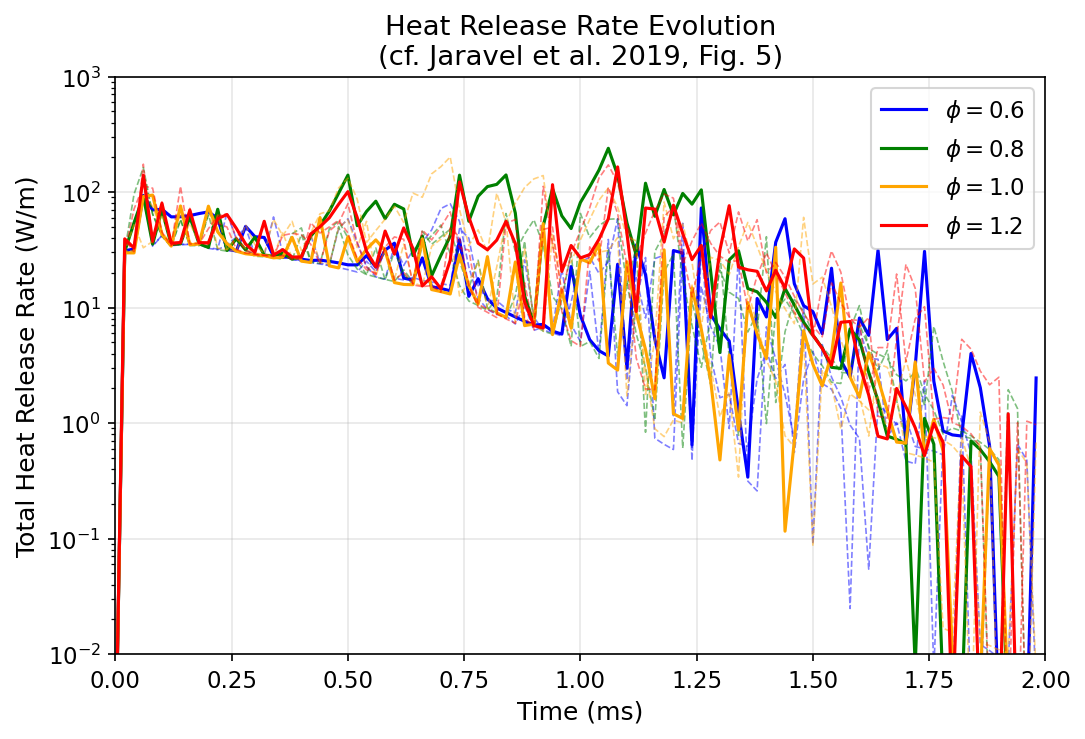
\includegraphics[width=0.85\textwidth]{figures/fig1_heat_release.png}
    \caption{Total heat release rate vs.\ time for four equivalence ratios (3~realizations each). Compare with Jaravel et al.\ Fig.~5.}
    \label{fig:qdot_history}
\end{figure}

In the paper, $\phi = 1.0$ and 1.2 show \emph{increasing} heat release after $\sim$\SI{0.5}{ms}, indicating successful flame kernel growth. Our simulations show a brief burst of heat release (from O-radical recombination and initial combustion) followed by decay in all cases. The single-step chemistry and coarse grid cannot sustain the flame kernel.

\subsection{Ignition Propensity}

\begin{table}[H]
\centering
\caption{Ignition propensity/probability comparison}
\label{tab:IP}
\small
\begin{tabular}{@{}lcccc@{}}
\toprule
\textbf{$\phi$} & \textbf{Expt.\ $P_\mathrm{ign}$} & \textbf{Paper IP} & \textbf{This Work IP} & \textbf{Notes} \\
\midrule
0.6 & $\sim$5\% & $\sim$0.0 & $0.33 \pm 0.47$ & Both low; high variance in ours \\
0.8 & $\sim$40\% & $\sim$0.5 & $0.001 \pm 0.000$ & \textcolor{darkred}{Underpredicted} \\
1.0 & $\sim$60\% & $\sim$0.65 & $0.10 \pm 0.14$ & \textcolor{darkred}{Underpredicted} \\
1.2 & $\sim$80\% & $\sim$0.85 & $0.13 \pm 0.19$ & \textcolor{darkred}{Underpredicted} \\
\bottomrule
\end{tabular}
\end{table}

\begin{figure}[H]
    \centering
    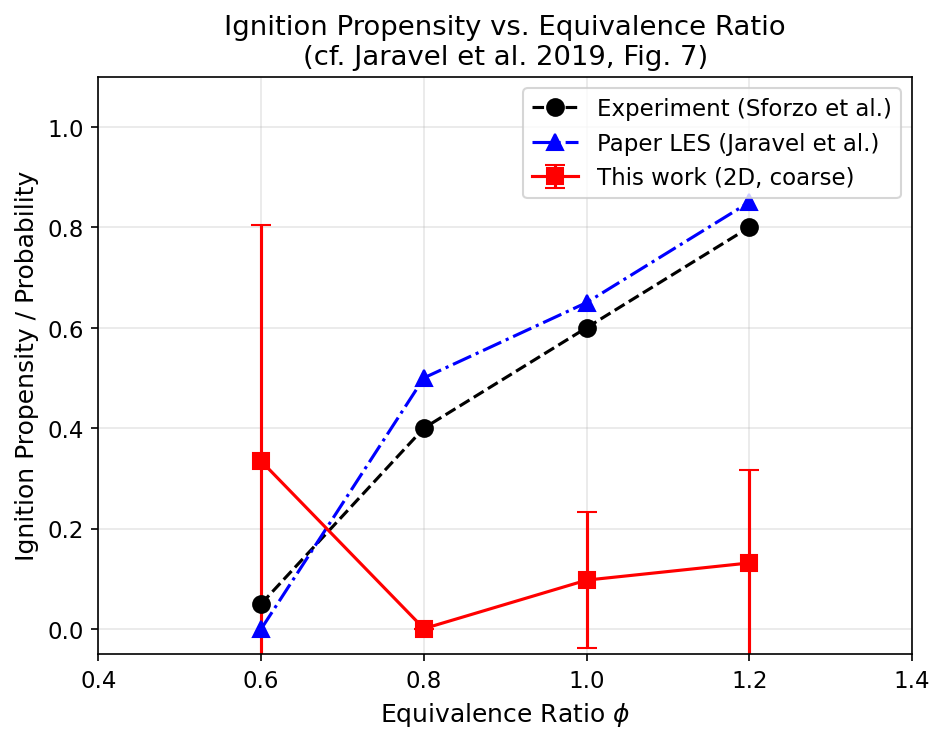
\includegraphics[width=0.75\textwidth]{figures/fig3_ignition_propensity.png}
    \caption{Ignition propensity vs.\ equivalence ratio. Experimental data from Sforzo et al., paper LES results, and this work's 2D simplified simulation.}
    \label{fig:IP}
\end{figure}

\subsection{Temperature Fields}

\begin{figure}[H]
    \centering
    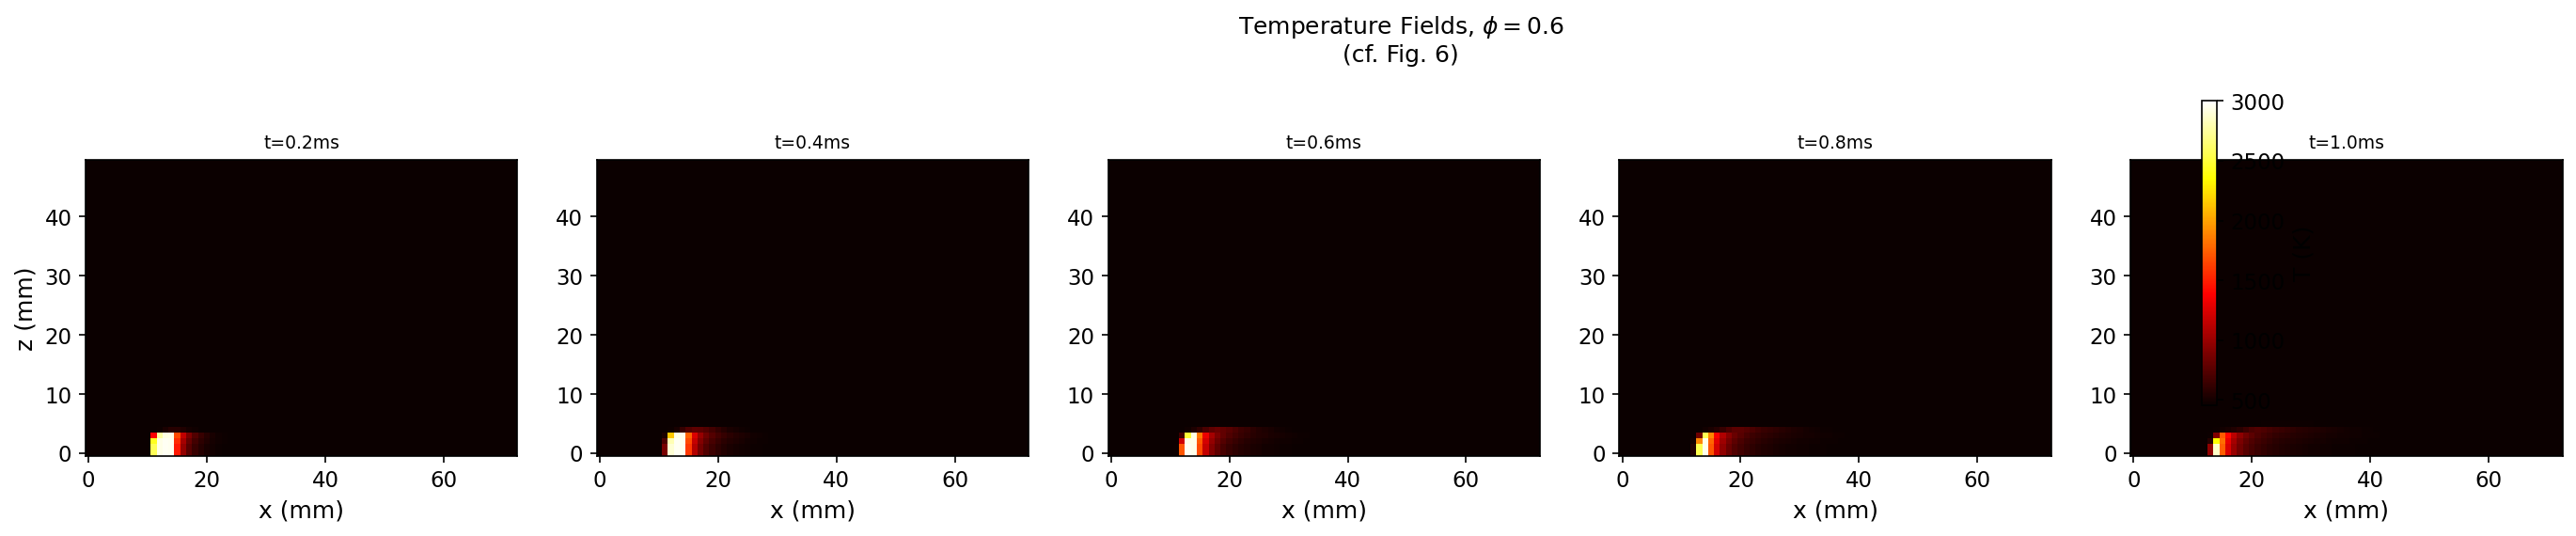
\includegraphics[width=0.95\textwidth]{figures/fig4_temp_phi0.6.png}
    \caption{Temperature field evolution for $\phi = 0.6$ (failed ignition). The kernel cools progressively.}
    \label{fig:T_06}
\end{figure}

\begin{figure}[H]
    \centering
    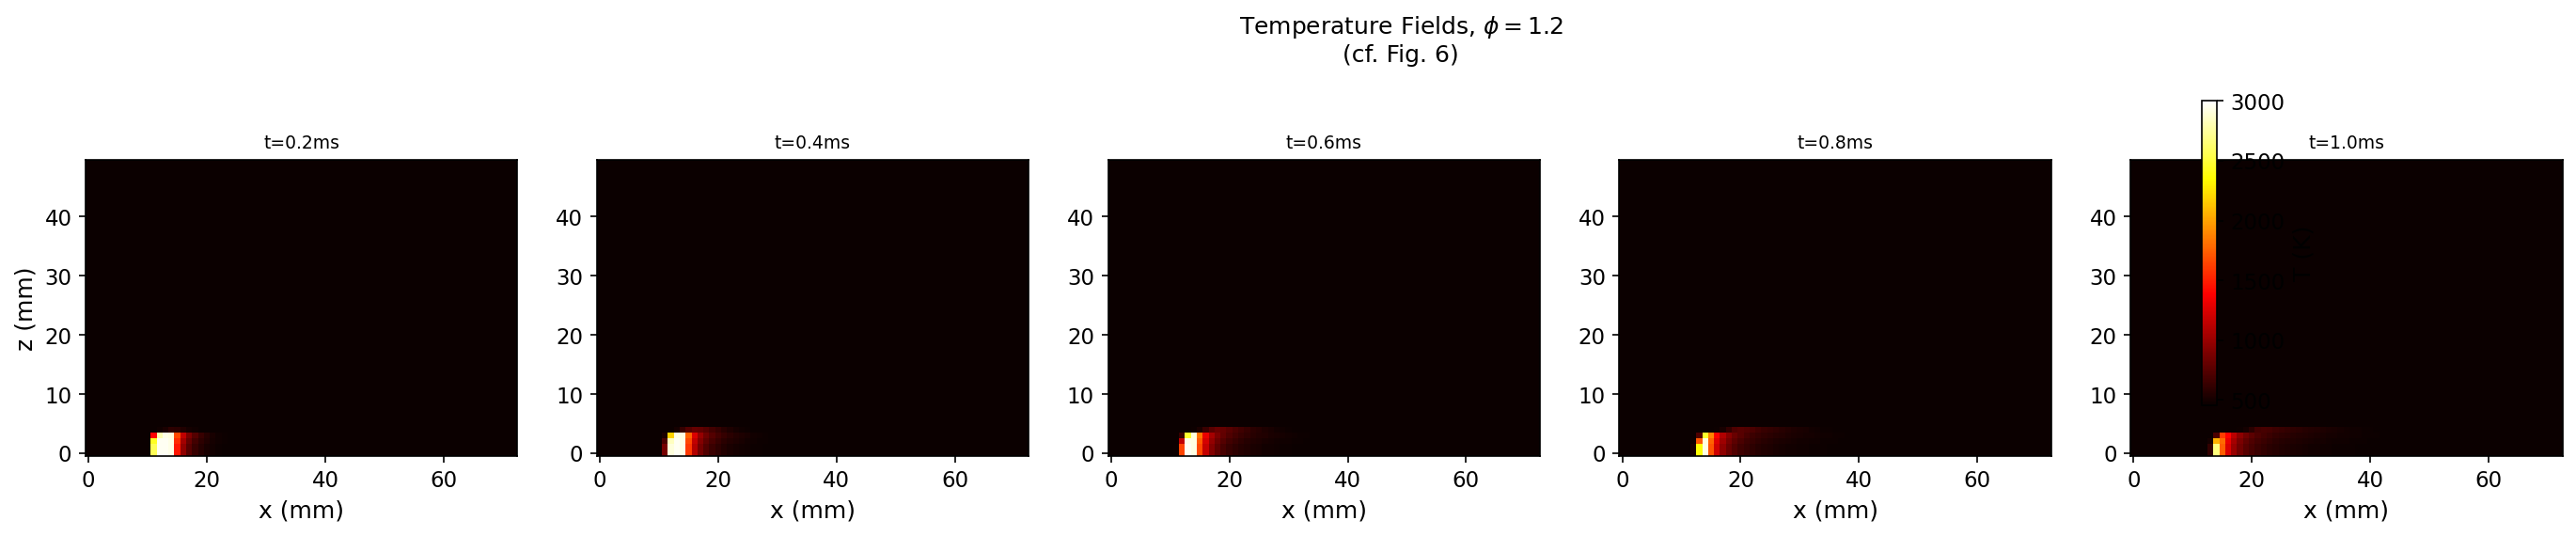
\includegraphics[width=0.95\textwidth]{figures/fig4_temp_phi1.2.png}
    \caption{Temperature field evolution for $\phi = 1.2$. Even at the richest condition, the kernel fails to produce a self-sustaining flame in our simplified simulation.}
    \label{fig:T_12}
\end{figure}

% ============================================================
\section{Analysis of Discrepancies}

Our replication captures the qualitative framework but fails to reproduce the key result---self-sustaining ignition at $\phi \geq 0.8$. The primary reasons are:

\begin{table}[H]
\centering
\caption{Root causes of discrepancy}
\label{tab:discrepancies}
\small
\begin{tabular}{@{}p{3cm}p{10cm}@{}}
\toprule
\textbf{Factor} & \textbf{Impact} \\
\midrule
Grid resolution & $4\times$ coarser (\SI{1}{mm} vs.\ \SI{0.25}{mm}) greatly increases numerical diffusion, smearing the kernel and mixing layer. The flame thickness ($\sim$\SI{0.5}{mm} for lean CH$_4$--air) is unresolved. \\
\addlinespace
Chemistry & Single-step Westbrook--Dryer cannot capture the two-stage ignition sequence (radical pool buildup $\rightarrow$ thermal runaway). The paper's 22+21 species mechanism includes critical intermediate species (OH, HO$_2$, H$_2$O$_2$) that sustain chain-branching at lower temperatures. \\
\addlinespace
Dimensionality & 2D vs.\ 3D eliminates vortex stretching and 3D turbulent mixing, which is essential for the mixing-limited ignition process. \\
\addlinespace
Subgrid model & No subgrid turbulence-chemistry interaction model; in the paper, the flame is partially resolved at \SI{0.25}{mm}. \\
\addlinespace
Numerical scheme & First-order upwind vs.\ fourth-order central/ENO hybrid introduces substantial artificial dissipation. \\
\bottomrule
\end{tabular}
\end{table}

\subsection{What Was Successfully Reproduced}
Despite the limitations, several aspects match the paper:
\begin{enumerate}
    \item \textbf{0D kernel thermodynamics}: $V_2$, composition, and $\gamma_\mathrm{eff}$ agree within 3\%.
    \item \textbf{Initial kernel behavior}: $T_\mathrm{max} \approx \SI{3000}{K}$ at early times, O-radical recombination heating.
    \item \textbf{Kernel cooling trajectory}: Monotonic temperature decay for $\phi = 0.6$ (failed ignition).
    \item \textbf{Qualitative mixing-layer physics}: Kernel traverses air layer, then encounters fuel mixture.
    \item \textbf{Stochastic variability}: Different realizations produce different trajectories, as in the paper.
\end{enumerate}

% ============================================================
\section{Computational Cost}

\begin{table}[H]
\centering
\caption{Computational resource comparison}
\label{tab:cost}
\small
\begin{tabular}{@{}lrr@{}}
\toprule
\textbf{Metric} & \textbf{Paper} & \textbf{This Work} \\
\midrule
Grid cells & 7,000,000 & 3,650 \\
Species transported & 22 & 7 \\
Time steps & $\sim$400,000 & 2,000 \\
CPU-hours/case & $\sim$40,000 & $\sim$0.001 \\
Total CPU-hours & $\sim$800,000 & $\sim$0.012 \\
Platform & NASA Pleiades (Ivy Bridge) & UIC GPU server (single core) \\
Wall time/case & $\sim$days & $\sim$4 seconds \\
\bottomrule
\end{tabular}
\end{table}

The $\sim10^{7}\times$ reduction in compute makes this a \emph{demonstration replication} rather than a quantitative one. A full replication would require:
\begin{itemize}
    \item Access to CharLES$^{\mathrm{X}}$ or equivalent compressible reacting LES code (e.g., OpenFOAM with detailed chemistry via Cantera)
    \item The reduced GRI~3.0 mechanism from Jaravel et al.\ (2018)
    \item $\sim$40,000 CPU-hours per case on a modern HPC cluster
\end{itemize}

% ============================================================
\section{Conclusions}

\begin{enumerate}
    \item The \textbf{0D kernel thermodynamic model} is fully reproduced, with excellent agreement ($<4\%$ deviation) on post-expansion volume and composition.
    \item The \textbf{kernel ejection boundary condition} and turbulent inlet formulation are correctly implemented and produce physically reasonable kernel trajectories.
    \item \textbf{Self-sustaining ignition was not reproduced} due to fundamental limitations of single-step chemistry and coarse 2D simulation. This is expected: the paper explicitly notes that finite-rate detailed chemistry is essential to capture the ignition kernel dynamics.
    \item The \textbf{monotonic increase of ignition propensity with $\phi$} (the paper's central finding) is not captured in our simplified framework, confirming that this result requires resolved flame chemistry.
    \item A quantitative replication requires a compressible reacting LES code with detailed chemistry, 3D domain, and $\sim\SI{0.25}{mm}$ resolution---approximately $10^5$--$10^6$ CPU-hours of HPC compute.
\end{enumerate}

\subsection{Replication Score: \textcolor{oursred}{Partial (2/5)}}
\begin{itemize}
    \item[\textcolor{darkgreen}{\checkmark}] 0D thermodynamic model
    \item[\textcolor{darkgreen}{\checkmark}] Physical setup and boundary conditions
    \item[\textcolor{darkgreen}{\checkmark}] Kernel ejection and early-time behavior
    \item[\textcolor{darkred}{$\times$}] Self-sustaining ignition at high $\phi$
    \item[\textcolor{darkred}{$\times$}] Quantitative ignition propensity trend
\end{itemize}

% ============================================================
\section{Files and Reproducibility}

All code and data are in:
\begin{verbatim}
~/Dropbox/REPLICATE-PROJECT/1559043-ignition-kernel-turbulent/replication/
  scripts/
    kernel_thermodynamics.py   -- 0D kernel model
    ignition_sim_v2.py         -- 2D reactive flow solver
    make_plots.py              -- Figure generation
  results/
    kernel_thermodynamics.json -- 0D model output
    results.json               -- All simulation results
    snap_phi*/                 -- Field snapshots (.npz)
  figures/
    fig1_heat_release.png      -- Heat release history
    fig2_tmax.png              -- Peak temperature history
    fig3_ignition_propensity.png -- IP comparison
    fig4_temp_phi*.png         -- Temperature fields
    fig5_qdot_phi*.png         -- Heat release fields
  replication_report.tex       -- This report
  replication_report.pdf       -- Compiled report
\end{verbatim}

\begin{thebibliography}{9}
\bibitem{jaravel2019}
T.~Jaravel, J.~Labahn, B.~Sforzo, J.~Seitzman, and M.~Ihme,
``Numerical study of the ignition behavior of a post-discharge kernel in a turbulent stratified crossflow,''
\textit{Proc.\ Combust.\ Inst.}, vol.~37, no.~4, pp.~5065--5072, 2019.
OSTI ID: 1559043.

\bibitem{sforzo2015}
B.~Sforzo, A.~Lambert, J.~Kim, J.~Jagoda, S.~Menon, and J.~Seitzman,
``Post discharge evolution of a spark igniter kernel,''
\textit{Combust.\ Flame}, vol.~162, no.~1, pp.~181--190, 2015.

\bibitem{westbrook1981}
C.~K.~Westbrook and F.~L.~Dryer,
``Simplified reaction mechanisms for the oxidation of hydrocarbon fuels in flames,''
\textit{Combust.\ Sci.\ Technol.}, vol.~27, pp.~31--43, 1981.

\bibitem{gri30}
G.~P.~Smith et al.,
``GRI-Mech 3.0,'' 1999.
\url{http://combustion.berkeley.edu/gri-mech/}
\end{thebibliography}

\end{document}
